%%%%%%%%%%%%%%%%%%%%%%%%%%%%%%%%%%%%%%%%%
% Lachaise Assignment
% LaTeX Template
% Version 1.0 (26/6/2018)
%
% This template originates from:
% http://www.LaTeXTemplates.com
%
% Authors:
% Marion Lachaise & François Févotte
% Vel (vel@LaTeXTemplates.com)
%
% License:
% CC BY-NC-SA 3.0 (http://creativecommons.org/licenses/by-nc-sa/3.0/)
% 
%%%%%%%%%%%%%%%%%%%%%%%%%%%%%%%%%%%%%%%%%

%----------------------------------------------------------------------------------------
%	PACKAGES AND OTHER DOCUMENT CONFIGURATIONS
%----------------------------------------------------------------------------------------

\documentclass{article}

%%%%%%%%%%%%%%%%%%%%%%%%%%%%%%%%%%%%%%%%%
% Lachaise Assignment
% Structure Specification File
% Version 1.0 (26/6/2018)
%
% This template originates from:
% http://www.LaTeXTemplates.com
%
% Authors:
% Marion Lachaise & François Févotte
% Vel (vel@LaTeXTemplates.com)
%
% License:
% CC BY-NC-SA 3.0 (http://creativecommons.org/licenses/by-nc-sa/3.0/)
% 
%%%%%%%%%%%%%%%%%%%%%%%%%%%%%%%%%%%%%%%%%

%----------------------------------------------------------------------------------------
%	PACKAGES AND OTHER DOCUMENT CONFIGURATIONS
%----------------------------------------------------------------------------------------

\usepackage{amsmath,amsfonts,stmaryrd,amssymb} % Math packages
\usepackage[dvipsnames]{xcolor}
\usepackage{enumerate} % Custom item numbers for enumerations
\usepackage{hyperref}
\usepackage[ruled,vlined]{algorithm2e} % Algorithms

\usepackage[framemethod=tikz]{mdframed} % Allows defining custom boxed/framed environments

\usepackage{listings} % Required for insertion of code

\newcommand{\randomcolor}{%
  \definecolor{randomcolor}{RGB}
   {
    \pdfuniformdeviate 256,
    \pdfuniformdeviate 256,
    \pdfuniformdeviate 256
   }%
  \color{randomcolor}%
}

\definecolor{codegreen}{rgb}{0,0.6,0}
\definecolor{codegray}{rgb}{0.5,0.5,0.5}
\definecolor{codepurple}{rgb}{0.58,0,0.82}
\definecolor{backcolour}{rgb}{1,1,1}
\lstdefinestyle{mystyle}{
    backgroundcolor=\color{backcolour},   
    commentstyle=\color{codegreen},
    keywordstyle=\color{magenta},
    numberstyle=\tiny\color{codegray},
    stringstyle=\color{codepurple},
    basicstyle=\ttfamily\footnotesize,
    breakatwhitespace=false,         
    breaklines=true,                 
    captionpos=b,                    
    keepspaces=true,                 
    numbers=left,                    
    numbersep=5pt,                  
    showspaces=false,                
    showstringspaces=false,
    showtabs=false,                  
    tabsize=2
}
\renewcommand{\lstlistingname}{Código}% Listing -> Algorithm
\lstset{style=mystyle}


%\usepackage{listings} % File listings, with syntax highlighting
%\lstset{
%	basicstyle=\ttfamily, % Typeset listings in monospace font
%}

%----------------------------------------------------------------------------------------
%	DOCUMENT MARGINS
%----------------------------------------------------------------------------------------

\usepackage{geometry} % Required for adjusting page dimensions and margins

\geometry{
	paper=a4paper, % Paper size, change to letterpaper for US letter size
	top=2.5cm, % Top margin
	bottom=3cm, % Bottom margin
	left=2.5cm, % Left margin
	right=2.5cm, % Right margin
	headheight=14pt, % Header height
	footskip=1.5cm, % Space from the bottom margin to the baseline of the footer
	headsep=1.2cm, % Space from the top margin to the baseline of the header
	%showframe, % Uncomment to show how the type block is set on the page
}

%----------------------------------------------------------------------------------------
%	FONTS
%----------------------------------------------------------------------------------------

\usepackage[utf8]{inputenc} % Required for inputting international characters
\usepackage[T1]{fontenc} % Output font encoding for international characters

\usepackage{XCharter} % Use the XCharter fonts
\usepackage{pgfplots}
\usepackage{multicol}
%----------------------------------------------------------------------------------------
%	COMMAND LINE ENVIRONMENT
%----------------------------------------------------------------------------------------

% Usage:
% \begin{commandline}
%	\begin{verbatim}
%		$ ls
%		
%		Applications	Desktop	...
%	\end{verbatim}
% \end{commandline}

\mdfdefinestyle{commandline}{
	leftmargin=10pt,
	rightmargin=10pt,
	innerleftmargin=15pt,
	middlelinecolor=black!50!white,
	middlelinewidth=2pt,
	frametitlerule=false,
	backgroundcolor=black!5!white,
	frametitle={Command Line},
	frametitlefont={\normalfont\sffamily\color{white}\hspace{-1em}},
	frametitlebackgroundcolor=black!50!white,
	nobreak,
}

% Define a custom environment for command-line snapshots
\newenvironment{commandline}{
	\medskip
	\begin{mdframed}[style=commandline]
}{
	\end{mdframed}
	\medskip
}

%----------------------------------------------------------------------------------------
%	FILE CONTENTS ENVIRONMENT
%----------------------------------------------------------------------------------------

% Usage:
% \begin{file}[optional filename, defaults to "File"]
%	File contents, for example, with a listings environment
% \end{file}

\mdfdefinestyle{file}{
	innertopmargin=1.6\baselineskip,
	innerbottommargin=0.8\baselineskip,
	topline=false, bottomline=false,
	leftline=false, rightline=false,
	leftmargin=2cm,
	rightmargin=2cm,
	singleextra={%
		\draw[fill=black!10!white](P)++(0,-1.2em)rectangle(P-|O);
		\node[anchor=north west]
		at(P-|O){\ttfamily\mdfilename};
		%
		\def\l{3em}
		\draw(O-|P)++(-\l,0)--++(\l,\l)--(P)--(P-|O)--(O)--cycle;
		\draw(O-|P)++(-\l,0)--++(0,\l)--++(\l,0);
	},
	nobreak,
}

% Define a custom environment for file contents
\newenvironment{file}[1][File]{ % Set the default filename to "File"
	\medskip
	\newcommand{\mdfilename}{#1}
	\begin{mdframed}[style=file]
}{
	\end{mdframed}
	\medskip
}

%----------------------------------------------------------------------------------------
%	NUMBERED QUESTIONS ENVIRONMENT
%----------------------------------------------------------------------------------------

% Usage:
% \begin{question}[optional title]
%	Question contents
% \end{question}

\mdfdefinestyle{question}{
	innertopmargin=1.2\baselineskip,
	innerbottommargin=0.8\baselineskip,
	roundcorner=5pt,
	nobreak,
	singleextra={%
		\draw(P-|O)node[xshift=1em,anchor=west,fill=white,draw,rounded corners=5pt]{%
		Pregunta \theQuestion\questionTitle};
	},
}

\newcounter{Question} % Stores the current question number that gets iterated with each new question

% Define a custom environment for numbered questions
\newenvironment{question}[1][\unskip]{
	\bigskip
	\stepcounter{Question}
	\newcommand{\questionTitle}{~#1}
	\begin{mdframed}[style=question]
}{
	\end{mdframed}
	\medskip
}

%----------------------------------------------------------------------------------------
%	WARNING TEXT ENVIRONMENT
%----------------------------------------------------------------------------------------

% Usage:
% \begin{warn}[optional title, defaults to "Warning:"]
%	Contents
% \end{warn}

\mdfdefinestyle{warning}{
	topline=false, bottomline=false,
	leftline=false, rightline=false,
	nobreak,
	singleextra={%
		\draw(P-|O)++(-0.5em,0)node(tmp1){};
		\draw(P-|O)++(0.5em,0)node(tmp2){};
		\fill[black,rotate around={45:(P-|O)}](tmp1)rectangle(tmp2);
		\node at(P-|O){\color{white}\scriptsize\bf !};
		\draw[very thick](P-|O)++(0,-1em)--(O);%--(O-|P);
	}
}

% Define a custom environment for warning text
\newenvironment{warn}[1][Warning:]{ % Set the default warning to "Warning:"
	\medskip
	\begin{mdframed}[style=warning]
		\noindent{\textbf{#1}}
}{
	\end{mdframed}
}

%----------------------------------------------------------------------------------------
%	INFORMATION ENVIRONMENT
%----------------------------------------------------------------------------------------

% Usage:
% \begin{info}[optional title, defaults to "Info:"]
% 	contents
% 	\end{info}

\mdfdefinestyle{info}{%
	topline=false, bottomline=false,
	leftline=false, rightline=false,
	nobreak,
	singleextra={%
		\fill[black](P-|O)circle[radius=0.4em];
		\node at(P-|O){\color{white}\scriptsize\bf i};
		\draw[very thick](P-|O)++(0,-0.8em)--(O);%--(O-|P);
	}
}

% Define a custom environment for information
\newenvironment{info}[1][Info:]{ % Set the default title to "Info:"
	\medskip
	\begin{mdframed}[style=info]
		\noindent{\textbf{#1}}
}{
	\end{mdframed}
}
 % Include the file specifying the document structure and custom commands

%----------------------------------------------------------------------------------------
%	ASSIGNMENT INFORMATION
%----------------------------------------------------------------------------------------

\title{ITC-ADA-C1-2023: Assignment \#3} % Title of the assignment

\author{Luis Ballado\\ \texttt{luis.ballado@cinvestav.mx}} % Author name and email address

\date{CINVESTAV UNIDAD TAMAULIPAS --- \today} % University, school and/or department name(s) and a date

%----------------------------------------------------------------------------------------

\begin{document}

\maketitle % Print the title

%----------------------------------------------------------------------------------------
%	INTRODUCTION
%----------------------------------------------------------------------------------------

\section{Considerando el algoritmo recursivo mostrado a continuación, responda las siguientes preguntas}

\begin{center}
  \begin{minipage}{0.7\linewidth} % Adjust the minipage width to accomodate for the length of algorithm lines
    \begin{algorithm}[H] 
      \SetKwInOut{Input}{entrada}\SetKwInOut{Output}{salida}
      \Input{Un arreglo $A[0..n-1]$ de números reales}
      \DontPrintSemicolon
      \caption{Algoritmo Misterio}
      \label{alg:loop}
      \If{n==1}{
        return A[0];
      }\Else{
        $temp \gets Misterio(A[0..n-2])$\\
        \If{temp <= A[n-1]}{
          return temp;
        }\Else{
          return A[n-1];
        }
      }
    \end{algorithm}
  \end{minipage}
\end{center}

\begin{question}
  \textbf{¿Qué calcula el algoritmo?}
  
  %se responde aquí
  \textit{El algoritmo recursivo calcula el elemento de minimo valor del arreglo}
    
\end{question}

\begin{question}
  \textbf{¿Cuál es el parámetro que indica el tamaño de la entrada del algoritmo?}
    %se responde aquí
  \textit{n, siendo este el tamaño del arreglo de entrada. Apartir de este valor se puede llegar al caso base.}
    
\end{question}

\begin{question}
  \textbf{¿Cuál es la operación básica del algoritmo?}
  %se responde aquí
  
  \textit{La comparación es la operación básica de tiempo constante $O(1)$ en cada llamada, el algoritmo compara el valor minimo del subarreglo con el último elemento del subarreglo}
    
\end{question}
\begin{question}
  \textbf{¿Cuáles son el mejor caso y el peor caso para este algoritmo?}
    %se responde aquí
  \textit{El mejor caso ocurre cuando el valor minimo es encontrado en la primera llamada donde el arreglo de entrada es pequeño A[0] y seria de tiempo constante $O(1)$}\\
  \textit{El peor caso ocurre cuando el minimo valor es encontrado en la última llamada a la función. En este caso el algoritmo hace \textbf{n} llamadas a función, siendo n el tamaño del arreglo. Convirtiendose en una complejidad lineal $O(n)$}
    
\end{question}
\begin{question}
  \textbf{Proporcione una expresión matemática (relación de recurrencia), en función del tamaño de la entrada del algoritmo, que permita calcular cuántas veces se ejecuta la operación básica en este algoritmo.}\\
    %se responde aquí
  \textit{T(n) = 1 cuando n = 1}\\
  \textit{T(n) = T(n-1)+1 cuando n > 1}\\
  \textit{T(n-1)+1 = T(n-2)+2 = T(n-3)+3 podemos decir que la recurrencia esta expresada como: $T(n-i)+i$ al ser $n-i=0$ para llegar al caso base $n=i$}\\
  \textit{T(0)+n = n+1; por lo tanto $T(n) \in \Theta(n)$ }
\end{question}
\begin{question}
  \textbf{Resuelva la relación de recurrencia propuesta mediante substitución hacia atrás}\\
    %se responde aquí
  \textit{Partiendo de la relación propuesta: $T(n) = T(n-1)+O(1)$}\\
  \textit{$T(n)$ es el tiempo de complejidad del algoritmo para tamaños de entrada n, $T(n-1)$ es el tiempo de complejidad para tamaños $n-1$ }\\
  \textit{$O(1)$ tiempo de complejidad por las comparaciones. La relación de recurrencia mediante substitución hacia atrás:}\\
  $T(n)=T(n-1)+O(1)$\\
  $T(n)=(T(n-2)+O(1))+O(1)$\\
  $T(n)=(T(n-3)+O(1)+O(1))+O(1)$\\
  $T(n)=(T(n-4)+O(1)+O(1)+O(1))+O(1)$\\
  podemos concluir que $T(n) = (T(1)+O(1)+O(1)+...+O(1))+O(1))$ donde $T(n)$ es el tiempo de complejidad para un array de tamaño n, $T(1)$ es la complejidad para tamaño 1 por la comparación constante
\end{question}

\begin{question}
  \textbf{¿Cuál es la clase de eficiencia?}
    %se responde aquí
  \textit{$T(n) \in O(n)$}
    
\end{question}

\newpage
\section{Dado el problema de encontrar el determinante de una matriz A de nxn , desarrolle los siguiente puntos:}

\begin{question}
  \textbf{Programe las versiones iterativa y recursiva del algoritmo para resolver el problema}
  %se responde aquí
  %\textit{Respuesta aqui}
\end{question}

\subsection{Implementación}

Código completo repo github \url{https://raw.githubusercontent.com/luisballado/ADA/main/assignments/assignment_3/determinante.py}

Por la facilidad de leer argumentos de entrada y guardar a texto los resultados de las corridas de los códigos, cambie la implementación

Ejecutar desde una terminal, depende de la versión de python instalada desde el ordenador. Ya que se incluye una solución de la libreria de numpy para la verificación de resultados, es probable la instalación de la biblioteca con el uso de pip \textbf{\$ pip install numpy}

% Command-line "screenshot"
\begin{commandline}
	\begin{verbatim}
		$ python3.10 determinante.py -size 12 > 12.txt
	\end{verbatim}
\end{commandline}

% File contents
\begin{file}[determinante.py]
\begin{lstlisting}[language=Python]
#version recursiva    
def recursivo(matrix):
    
    n = len(matrix)

    #caso base
    if n == 1:
        return matrix[0][0]
    if n == 2:
        return matrix[0][0] * matrix[1][1] - matrix[0][1] * matrix[1][0]

    det = 0
    for i in range(n):
        sub_matrix = [row[:i] + row[i+1:] for row in matrix[1:]] 
        det += ((-1) ** i) * matrix[0][i] * recursivo(sub_matrix)

    return det

#version iterativa
def iterativo(matrix):
    determinant = 1
    n = len(matrix)
    for i in range(n):
        # Encontrar el valor maximo en la columna
        maxRow = i
        for j in range(i + 1, n):
            if abs(matrix[j][i]) > abs(matrix[maxRow][i]):
                maxRow = j
        # intercambiar el maximo valor con el valor actual
        if maxRow != i:
            matrix[i], matrix[maxRow] = matrix[maxRow], matrix[i]
            determinant *= -1

        # Multiplicar el determinante por la diagonal
        determinant *= matrix[i][i]
        
        # terminar si los elementos de la diagonal son ceros
        if matrix[i][i] == 0:
            return 0

        # Eliminar los elementos abajo de la diagonal
        for j in range(i + 1, n):
            if matrix[i][i] == 0:
                scale = 0
            else:
                scale = matrix[j][i] / matrix[i][i]
                
            for k in range(i, n):
                matrix[j][k] -= scale * matrix[i][k]
                
    return determinant

\end{lstlisting}
\end{file}

\begin{question}
  \textbf{Analice matemáticamente cada versión el algoritmo por separado usando las metodologías vistas en clase.}
    %se responde aquí
  \textit{versión recursiva $T(n) = T(n-1) + O(n^{2})$ donde $O(n^{2})$ es el tiempo de complejidad del calculo de las submatrices, y $T(n-1)$ tiempo de complejidad cuando se reduce la matriz $n-1$ en un análisis por cofactores}\\
  El tiempo de complejidad del cálculo de submatrices puede estar expresado por $O(n^{2})$ ya que cada elemento pertenece a la primera fila, se va creando una submatriz de tamaño reducido $n-1 x n-1$ para ir llegando al caso base.\\
  $T(n) = T(n-1)+O(n^{2})$\\
  $T(n) = (T(n-2)+ O(n^{2}))+O(n^{2})$\\
  hasta llegar al caso base\\
  $T(n) = (T(1) + O(n^{2})+O(n^{2})+...+O(n^{2})+O(n^{2}))$\\
  podemos concluir que $T(n) = T(1) + n*O(n^{2})$\\
  $T(n) = O(n^{3})$, pero para un peor caso donde la matriz es muy grande, \\el algoritmo en su versión recursiva $T(n) \in \Theta(n!)$

  

\end{question}

\begin{question}
  \textbf{En base a los resultados obtenidos en el punto anterior determine cuál de los dos algoritmos es más eficiente}
    %se responde aquí
  \textit{A pesar del crecimiento del orden polinomial, la versión iterativa tiene un mejor comportamiento contra su versión recursiva}
\end{question}

\begin{question}
  \textbf{Para cada uno de los dos algoritmos desarrollados aplique el método descrito en el apartado "Doubling ratio experiments" del libro Algorithms de Sedgewick y Wayne, generando instancias de tamaños 1000,2000,etc; hasta lograr un radio de $2^{b}$, ejecutando 20 pruebas con cada tamaño y con cada algoritmo. Registre sus resultados.}
    %se responde aquí
  \textit{Al ejecutar los algoritmos dentro del mismo programa y guardar los resultados en un archivo de texto con la salidad resultante de cada experimento, el orden de crecimiento factorial del algoritmo recursivo disparo la ejecución del análisis de una matriz de tamaño 24x24 llegando a no ser rentable para esperar el resultado}
\end{question}

\begin{question}
  \textbf{Para cada algoritmo comparado realice una tabla con 5 predicciones, posteriores al tamaño con que se logró obtener el radio $2^{b}$}
    %se responde aquí
  \begin{center}
    \begin{tabular}{||c c c||} 
      \hline
      TAMAÑO & Iterativa & Recursiva \\ [0.5ex] 
      \hline
      14x14 & 0.0391 ms & - \\
      \hline
      28x28 & 0.1227 ms & +7 días \\
      \hline
      56x56 & 0.4293 ms & 13 años \\
      \hline
      112x112 & 0.0052 s & $\infty$ \\
      \hline
      224x224 & 0.0208 s & $\infty$ \\
      \hline
    \end{tabular}
  \end{center}
\end{question}

\begin{question}
  \textbf{Para cada algoritmo comparado grafique los siguientes resultados de sus ejecuciones}
    %se responde aquí
  \textit{Los resultados obtenidos de las corridas de los algoritmos son las siguientes:}\\

  \begin{multicols}{2}
  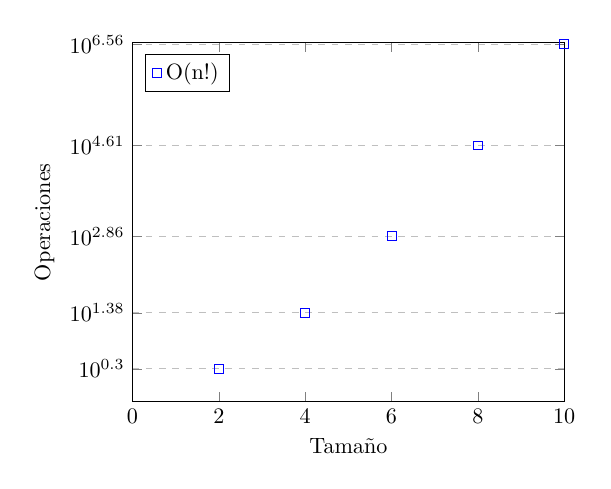
\begin{tikzpicture}[scale=0.80]
    \begin{semilogyaxis}[
        %title={Comparativa},
        xlabel={Tamaño},
        ylabel={Operaciones},
        xmin=0, xmax=10,
        ymin=0, ymax=3828800,
        xtick={0,2,4,6,8,10},
        ytick={0,2,24,720,40320,3628800},
        legend pos=north west,
        ymajorgrids=true,
        grid style=dashed,
      ]
      \addplot[
        color=blue,
        only marks,
        mark=square,
      ]
      coordinates {
        (0,0)(2,2)(4,24)(6,720)(8,40320)(10,3628800)
      };
      \legend{O(n!)}
    \end{semilogyaxis}
  \end{tikzpicture}

  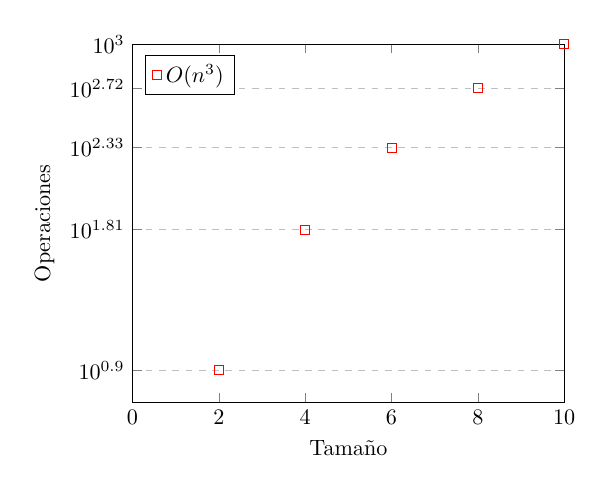
\begin{tikzpicture}[scale=0.80]
    \begin{semilogyaxis}[
        %title={Comparativa},
        xlabel={Tamaño},
        ylabel={Operaciones},
        xmin=0, xmax=10,
        ymin=0, ymax=1000,
        xtick={0,2,4,6,8,10},
        ytick={0,8,64,216,521,1000},
        legend pos=north west,
        ymajorgrids=true,
        grid style=dashed,
      ]
      \addplot[
        color=red,
        only marks,
        mark=square,
      ]
      coordinates {
        (0,0)(2,8)(4,64)(6,216)(8,521)(10,1000)
      };
      \legend{$O(n^{3})$}
    \end{semilogyaxis}
  \end{tikzpicture}
  \end{multicols}
  
  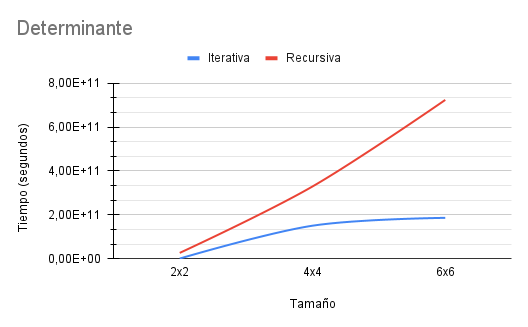
\includegraphics[scale=0.5]{grafico.png}
  
  \begin{center}
    \begin{tabular}{||c c c||} 
      \hline
      TAMAÑO & Iterativa & Recursiva \\ [0.5ex] 
      \hline\hline
      2x2 & 0.01120 ms & 0.00262 ms \\ 
      \hline
      4x4 & 0.01502 ms & 0.03290 ms \\
      \hline
      6x6 & 0.01859 ms & 0.00072 ms \\
      \hline
      8x8 & 0.02670 ms & 0.05136 ms \\
      \hline
      12x12 & 0.03695 ms & 654000 ms \\
      \hline
      14x14 & - & - \\
      \hline
      16x16 & - & - \\
      \hline
      24x24 & - & - \\
      \hline
    \end{tabular}
  \end{center}

  para la corrida de tamaño 24x24 a pesar de que el tiempo de ejecución fue de aproximadamente 5 horas, paré el proceso debido a que no tenia fin
\end{question}

\begin{question}
  \textbf{Con base en los experimentos realizados y considerando un tiempo máximo de ejecución sobre su computadora de 7 días, ¿Cuál es el tamaño máximo de entrada que puede resolver cada algoritmo analizado?}
    %se responde aquí
  \textbf{Iterativo} \textit{En su versión iterativa el algoritmo tiene una complejidad $O(n^{3})$. Y asumiendo que de entrada es una matriz de más de mil elementos, para cada iteración el algoritmo requerá $1000^{3}$ operaciones y considerando que las ejecuciones por segundo dependen del poder de procesamiendo de la máquina a usar, digamos que puede ejecutar $10^{9}$ operaciones por segundo. Calculariamos el numero de operaciones en un periodo de 7 dias como 7dias * 24horas * 60minutos * 60segundos = 604800 segundos; si los multiplicamos por el número de ejecuciones por segundo aproximadamente $6.048 * 10^{4}$ iteraciones en 7 días}\\
  \textbf{Recursivo} \textit{En su versión recursiva el algoritmo tiene una complejidad $O(n!)$ lo que nos dice es que el numero de operaciones que ejecuta el algoritmo crece en un rango proporcional al factorial de la entrada de la matriz. Para largas entradas las operaciones son extremadamente largas y no practicas de realizar. Para una entrada de n = 10, el número de operaciones rondaria en 3,628,800, pero si doblamos la entrada las operaciones se disparán a 2,432,902,000,000,000,000 lo cual es muy lejos del rango que pueda realizar en 7 días}
\end{question}

\begin{question}
  \textbf{Conclusiones respecto al orden de crecimiento de cada algoritmo observado empíricamente y constrástelas contra los resultados de sus análisis matemático}
    %se responde aquí
  \textit{Debido a los tiempos de ejecución altos para los cálculos de matrices con grandes tamaños los experimientos fueron reducidos a tamaños pequeños, pero de igual forma se pudo apreciar el mejor comportamiento para la versión iterativa del calculo de una determinante. En la práctica la ejecución de algoritmos de orden factorial es una mala idea por el crecimiento rápido y sólo es apreciable con entradas pequeñas.}
\end{question}

\section{Referencias}

\begin{itemize}
\item LATEX Documentación - \url{https://www.overleaf.com/learn}
\item RELACIONES DE RECURRENCIA - \url{https://medium.com/@matematicasdiscretaslibro/cap%C3%ADtulo-10-relaciones-de-recurrencia-7fe23208184}
\item Cálculo de determinantes - \url{https://www.uv.mx/personal/aherrera/files/2014/08/08d.-MENORES-COFACTORES-Y-DETERMINANTES.pdf}
\item Sedgewick And Wayne - Algorithms 4th Edición
\item Manejo de Listas python - \url{https://uniwebsidad.com/libros/algoritmos-python/capitulo-7/listas}
\item Determiante de una Matriz - \url{https://www.geeksforgeeks.org/determinant-of-a-matrix/}
\item What is the best algorithm to find a determinant of a matrix? - \url{https://stackoverflow.com/questions/2435133/what-is-the-best-algorithm-to-find-a-determinant-of-a-matrix}

\end{itemize}

\end{document}

